\chapter{Expansion of the Parameter Space}
\label{chap: A_s}

Now that we have a comprehensive set of convenience functions with which to
configure CAMB, we can easily obtain the theoretical power spectra we need in
order to demonstrate our solution to the neutrino difficulties introduced in
section~\ref{sec: neutrino_problem}. This chapter will motivate the inclusion 
of the additional parameter $A_s$ in the evolution mapping framework.
Because the focus of this thesis is regression rather than theory,
we will merely show that $A_s$ contains information relevant to the impact of
massive neutrinos. Then, the GPR should, in principle, be able to optimize its
use to predict power spectra.

% Maybe it would make more sense to have the large cass-L chapter focus on the
% creation of a massless-neutrino emulator and THEN a smaller chapter focusing
% on all the changes necessary for it to become a massive-neutrino emulator.
% BUT! As of 25-08-23, I'm running way behind on writing actual content for
% this thesis. I can't risk redoing all the section headers again. We're
% going to proceed under the current scheme and MAYBE allow ourselves to redo
% it shortly before submission.

\section{Equation to be Solved}

% Redo section title

\textcolor{orange}{Remember to explain \textit{why} the prediction of these 
asymptotes means that $A_s$ will capture most of the unruly behavior of 
neutrinos. What theory motivates such a judgment? Or are we only guessing?}

We begin with the second proposal from section~\ref{sec: neutrino_problem}:
to approximate the power spectrum of a massive-neutrino cosmology, we
combine the
power spectrum of its MEMNeC with an approximation of the ratio
between the two:

\begin{equation}
\label{eq: MEMNeC_approx}
P_\nu(k) \approx \de^* (k) P_0 (k)
,\end{equation}

The essence of this chapter is to increase the accuracy in our $P_\nu(k)$
predictions by estimating the true $\de(k)$. Specifically, we are interested
in how the true $\de(k)$ deviates from $\de^*(k)$. Therefore, we pay special
attention to the quantity:

\begin{equation}
\label{eq: ee}
\ee (k) \equiv \frac{\de(k)}{\de^*(k)}
\end{equation}

To simplify the discussion, we will concentrate on the small-scale limit of 
this ratio $\el$

\begin{equation}
\el \equiv \lim_{k \rightarrow \infty} \ee(k)
\end{equation}

If we can estimate $\el$ accurately, then in principle our task 
is complete, because the slope toward smaller $k$ values is
even and analytically predictable. \textcolor{green}{Can I refer the reader to
 a paper on this?}

\section{Proposed Fitting Functions}
 
In order to explore this limit concretely, we will use the Aletheia models as
our test cases. This means that we can rewrite definition~\ref{eq: ee} as:

\begin{equation}
\label{eq: ee}
\ee_i (k) \equiv \frac{\de_\text{model i}(k)}{\de_\text{model 0}(k)}
\end{equation}

\textcolor{orange}{This section, like the ``Convenience Functions'' section
from chapter 2, should anticipate CL: we should talk about the
code that we have written in order to explore these ratios, which one can find
in} \verb|camb_interface.py|.

To study the behavior of $\ee_i$, we developed the \verb|camb_interface.py|
function \verb|model_ratios|. This function accepts a single snap
index\footnote{remember that there are four snaps for each model, and snap 
four always corresponds to $z = 0$} and a set of power spectra nearly in the
format returned by \verb|boltzmann_battery|, but without the $\omega_\nu$ 
layer.\footnote{for explanations of the
remaining function parameters, we refer the reader to the docstring} it
computes and plots all of the $\ee_i$ spectra in the input set. We show an
example of its output in figure~\ref{fig: model_ratios_demo}. This function
is recommended for any users seeking to improve the characterization of
$\ee_i$.

% The following plots were generated with divergence_asymptotes.ipynb
\begin{figure}[ht!]
    \begin{subfigure}{0.45 \textwidth}
    \centering
 		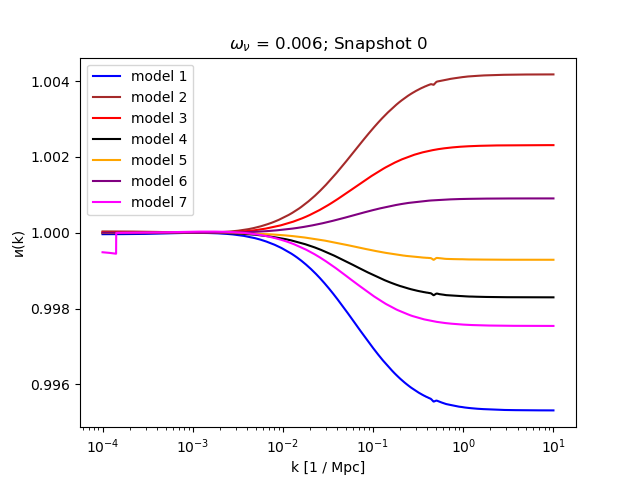
\includegraphics[width=\textwidth]{chap3/model_ratios}
 		\cprotect\caption{Example output of \verb|model_ratios|.}
 		\label{fig: model_ratios_demo}
    \end{subfigure}
    \begin{subfigure}{0.45 \textwidth}
    \centering
 		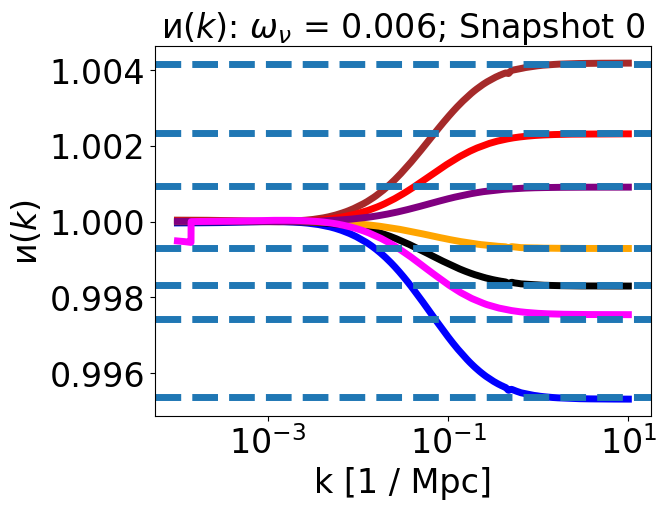
\includegraphics[width=\textwidth]{chap3/predictor_success}
 		\caption{With asymptote predictions.}
 		\label{fig: ee_prediction_demo}
    \end{subfigure}
        \centering
    \caption[$\ee$]
    		{Model ratios
    		\textcolor{red}{Would it have been better if I just included the
    		right plot and no left plot?}}
    \label{fig: model_ratios}
\end{figure}

\textcolor{orange}{The above paragraph only describes the function in the
case ``massive=`x'''}

We fit the asymptotes with a log. An example of its effect is visualized in
figure~\ref{fig: ee_prediction_demo}.


\section{Testing Functions}

Now we need to make sure that our prediction works well in other cases, not
just for the canonical Aletheia models.

We produce two sets of test cases, one for random cosmologies, one for
random cosmologies with $A_s$ fixed. Specifically, we only randomize
evolution parameters.

The \verb|get_As_matched_cosmology| function.
The \verb|get_random_cosmology| function.

In producing asymptote plots, we find that our predictions line up quite well,
but not perfectly. This may indicate that our parametrization is insufficient.
In other words, we may need additional cosmological parameters besides the
$A_s$ and $\omega_\nu$ and in order to fully characterize the impact of
massive neutrinos on the power spectrum.

However, the imperfect performance of our predictions may also simply
indicate that the final form of our asymptote predictions (equation XXY) is
only an approximation of some true (or at least more accurate) relationship
between $A_s$, $\omega_\nu$, and the small-scale suppression of the power
spectrum. A symbolic regression investigation could prove highly effective at
resolving this ambiguity by efficiently searching out improved formulas. 
However, we do not consider this a promising avenue
for the continuation of this work (see section~\ref{sec: future_work} for our
recommendations), because the error on our predictions is so low. The error
is so low here that we do not believe the imperfect predictions to
significantly detract from the performance of the emulator.

\section{Summary of Findings}

% I'm not sure if this section will survive, we'll see how big the conclusion
% here ends up being.

So, our massive-neutrino emulator will be trained over six cosmological
parameters: $\omega_b$, $\omega_c$, $n_s$, $\sigma_{12}$, $A_s$, and
$\omega_\nu$. In other words, to predict a power
spectrum $\hat{\vec{y}}$, the emulator will accept as an input $\vec{x}$
these six parameters.

%s Now segue into the next chapter

We just need to add $A_s$ to the set of cosmological parameters
over which we train our GPR and then we can treat $\omega_\nu$ like a shape
parameter. Expansion of the parameter space represents the single most 
important novel step in this work. The remaining chapters will
focus on the integration of this new approach into a beginner-friendly
emulation code.
